\PassOptionsToPackage{unicode=true}{hyperref} % options for packages loaded elsewhere
\PassOptionsToPackage{hyphens}{url}
%
\documentclass[
]{article}
\usepackage{lmodern}
\usepackage{amssymb,amsmath}
\usepackage{ifxetex,ifluatex}
\ifnum 0\ifxetex 1\fi\ifluatex 1\fi=0 % if pdftex
  \usepackage[T1]{fontenc}
  \usepackage[utf8]{inputenc}
  \usepackage{textcomp} % provides euro and other symbols
\else % if luatex or xelatex
  \usepackage{unicode-math}
  \defaultfontfeatures{Scale=MatchLowercase}
  \defaultfontfeatures[\rmfamily]{Ligatures=TeX,Scale=1}
\fi
% use upquote if available, for straight quotes in verbatim environments
\IfFileExists{upquote.sty}{\usepackage{upquote}}{}
\IfFileExists{microtype.sty}{% use microtype if available
  \usepackage[]{microtype}
  \UseMicrotypeSet[protrusion]{basicmath} % disable protrusion for tt fonts
}{}
\makeatletter
\@ifundefined{KOMAClassName}{% if non-KOMA class
  \IfFileExists{parskip.sty}{%
    \usepackage{parskip}
  }{% else
    \setlength{\parindent}{0pt}
    \setlength{\parskip}{6pt plus 2pt minus 1pt}}
}{% if KOMA class
  \KOMAoptions{parskip=half}}
\makeatother
\usepackage{xcolor}
\IfFileExists{xurl.sty}{\usepackage{xurl}}{} % add URL line breaks if available
\IfFileExists{bookmark.sty}{\usepackage{bookmark}}{\usepackage{hyperref}}
\hypersetup{
  pdftitle={Mushroom Classification},
  pdfauthor={Andreas Klaß, Cornelia Gruber, Felix Langer, Viktoria Szabo},
  pdfborder={0 0 0},
  breaklinks=true}
\urlstyle{same}  % don't use monospace font for urls
\usepackage[margin=1in]{geometry}
\usepackage{color}
\usepackage{fancyvrb}
\newcommand{\VerbBar}{|}
\newcommand{\VERB}{\Verb[commandchars=\\\{\}]}
\DefineVerbatimEnvironment{Highlighting}{Verbatim}{commandchars=\\\{\}}
% Add ',fontsize=\small' for more characters per line
\usepackage{framed}
\definecolor{shadecolor}{RGB}{248,248,248}
\newenvironment{Shaded}{\begin{snugshade}}{\end{snugshade}}
\newcommand{\AlertTok}[1]{\textcolor[rgb]{0.94,0.16,0.16}{#1}}
\newcommand{\AnnotationTok}[1]{\textcolor[rgb]{0.56,0.35,0.01}{\textbf{\textit{#1}}}}
\newcommand{\AttributeTok}[1]{\textcolor[rgb]{0.77,0.63,0.00}{#1}}
\newcommand{\BaseNTok}[1]{\textcolor[rgb]{0.00,0.00,0.81}{#1}}
\newcommand{\BuiltInTok}[1]{#1}
\newcommand{\CharTok}[1]{\textcolor[rgb]{0.31,0.60,0.02}{#1}}
\newcommand{\CommentTok}[1]{\textcolor[rgb]{0.56,0.35,0.01}{\textit{#1}}}
\newcommand{\CommentVarTok}[1]{\textcolor[rgb]{0.56,0.35,0.01}{\textbf{\textit{#1}}}}
\newcommand{\ConstantTok}[1]{\textcolor[rgb]{0.00,0.00,0.00}{#1}}
\newcommand{\ControlFlowTok}[1]{\textcolor[rgb]{0.13,0.29,0.53}{\textbf{#1}}}
\newcommand{\DataTypeTok}[1]{\textcolor[rgb]{0.13,0.29,0.53}{#1}}
\newcommand{\DecValTok}[1]{\textcolor[rgb]{0.00,0.00,0.81}{#1}}
\newcommand{\DocumentationTok}[1]{\textcolor[rgb]{0.56,0.35,0.01}{\textbf{\textit{#1}}}}
\newcommand{\ErrorTok}[1]{\textcolor[rgb]{0.64,0.00,0.00}{\textbf{#1}}}
\newcommand{\ExtensionTok}[1]{#1}
\newcommand{\FloatTok}[1]{\textcolor[rgb]{0.00,0.00,0.81}{#1}}
\newcommand{\FunctionTok}[1]{\textcolor[rgb]{0.00,0.00,0.00}{#1}}
\newcommand{\ImportTok}[1]{#1}
\newcommand{\InformationTok}[1]{\textcolor[rgb]{0.56,0.35,0.01}{\textbf{\textit{#1}}}}
\newcommand{\KeywordTok}[1]{\textcolor[rgb]{0.13,0.29,0.53}{\textbf{#1}}}
\newcommand{\NormalTok}[1]{#1}
\newcommand{\OperatorTok}[1]{\textcolor[rgb]{0.81,0.36,0.00}{\textbf{#1}}}
\newcommand{\OtherTok}[1]{\textcolor[rgb]{0.56,0.35,0.01}{#1}}
\newcommand{\PreprocessorTok}[1]{\textcolor[rgb]{0.56,0.35,0.01}{\textit{#1}}}
\newcommand{\RegionMarkerTok}[1]{#1}
\newcommand{\SpecialCharTok}[1]{\textcolor[rgb]{0.00,0.00,0.00}{#1}}
\newcommand{\SpecialStringTok}[1]{\textcolor[rgb]{0.31,0.60,0.02}{#1}}
\newcommand{\StringTok}[1]{\textcolor[rgb]{0.31,0.60,0.02}{#1}}
\newcommand{\VariableTok}[1]{\textcolor[rgb]{0.00,0.00,0.00}{#1}}
\newcommand{\VerbatimStringTok}[1]{\textcolor[rgb]{0.31,0.60,0.02}{#1}}
\newcommand{\WarningTok}[1]{\textcolor[rgb]{0.56,0.35,0.01}{\textbf{\textit{#1}}}}
\usepackage{longtable,booktabs}
% Allow footnotes in longtable head/foot
\IfFileExists{footnotehyper.sty}{\usepackage{footnotehyper}}{\usepackage{footnote}}
\makesavenoteenv{longtable}
\usepackage{graphicx,grffile}
\makeatletter
\def\maxwidth{\ifdim\Gin@nat@width>\linewidth\linewidth\else\Gin@nat@width\fi}
\def\maxheight{\ifdim\Gin@nat@height>\textheight\textheight\else\Gin@nat@height\fi}
\makeatother
% Scale images if necessary, so that they will not overflow the page
% margins by default, and it is still possible to overwrite the defaults
% using explicit options in \includegraphics[width, height, ...]{}
\setkeys{Gin}{width=\maxwidth,height=\maxheight,keepaspectratio}
\setlength{\emergencystretch}{3em}  % prevent overfull lines
\providecommand{\tightlist}{%
  \setlength{\itemsep}{0pt}\setlength{\parskip}{0pt}}
\setcounter{secnumdepth}{-2}
% Redefines (sub)paragraphs to behave more like sections
\ifx\paragraph\undefined\else
  \let\oldparagraph\paragraph
  \renewcommand{\paragraph}[1]{\oldparagraph{#1}\mbox{}}
\fi
\ifx\subparagraph\undefined\else
  \let\oldsubparagraph\subparagraph
  \renewcommand{\subparagraph}[1]{\oldsubparagraph{#1}\mbox{}}
\fi

% set default figure placement to htbp
\makeatletter
\def\fps@figure{htbp}
\makeatother


\title{Mushroom Classification}
\author{Andreas Klaß, Cornelia Gruber, Felix Langer, Viktoria Szabo}
\date{10.05.2020}

\begin{document}
\maketitle

\begin{figure}

{\centering 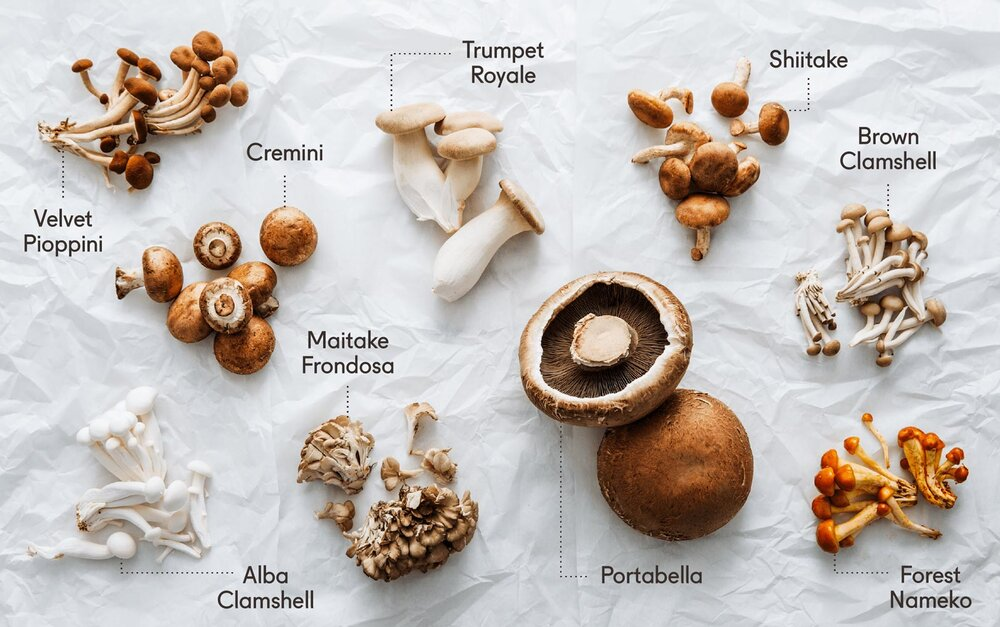
\includegraphics[width=1\linewidth]{images/mushrooms1} 

}

\caption{source: https://blog.goodeggs.com/blog/cooking-different-types-of-mushrooms}\label{fig:unnamed-chunk-1}
\end{figure}

Collecting mushrooms recently gained popularity (if you believe
Instagram influencers and mushroom picking blogs). Since mushrooms come
in many different colors and shapes, their fit or unfit for human
consumption is not necessarily obvious. Naturally, instead of asking
your grandparents for advice a statistical analysis is the way to go to
find out whether a mushroom is edible or poisonous given attributes
concerning the look or smell of a mushroom.

\hypertarget{mushroom-attributes}{%
\subsubsection{Mushroom attributes}\label{mushroom-attributes}}

Our main goal is to classify each mushroom into one of the two classes
``edible'' or ``poisonous''. For this task we can use various attributes
of a mushroom's cap, gill or stalk or attributes like the odor,
population or habitat of the mushroom. The cap shape for example can be
either ``bell'', ``conical'', ``convex'', ``flat'', ``knobbed'' or
``sunken'' (see figure below). The dataset contains 8124 observations
with 22 nominal features.

\begin{figure}

{\centering \includegraphics[width=0.49\linewidth,height=0.2\textheight]{images/parts-of-a-mushroom} \includegraphics[width=0.49\linewidth,height=0.2\textheight]{images/cap-shapes} 

}

\caption{source: https://www.mushroomdiary.co.uk/mushroom-identification/}\label{fig:unnamed-chunk-2}
\end{figure}

\hypertarget{dataset-overview}{%
\subsubsection{Dataset Overview}\label{dataset-overview}}

\begin{longtable}[]{@{}ll@{}}
\toprule
\begin{minipage}[b]{0.47\columnwidth}\raggedright
Variable\strut
\end{minipage} & \begin{minipage}[b]{0.47\columnwidth}\raggedright
Encoding\strut
\end{minipage}\tabularnewline
\midrule
\endhead
\begin{minipage}[t]{0.47\columnwidth}\raggedright
classes\strut
\end{minipage} & \begin{minipage}[t]{0.47\columnwidth}\raggedright
edible=e, poisonous=p\strut
\end{minipage}\tabularnewline
\begin{minipage}[t]{0.47\columnwidth}\raggedright
cap-shape\strut
\end{minipage} & \begin{minipage}[t]{0.47\columnwidth}\raggedright
bell=b, conical=c, convex=x, flat=f, knobbed=k, sunken=s\strut
\end{minipage}\tabularnewline
\begin{minipage}[t]{0.47\columnwidth}\raggedright
cap-surface\strut
\end{minipage} & \begin{minipage}[t]{0.47\columnwidth}\raggedright
fibrous=f, grooves=g, scaly=y, smooth=s\strut
\end{minipage}\tabularnewline
\begin{minipage}[t]{0.47\columnwidth}\raggedright
cap-color\strut
\end{minipage} & \begin{minipage}[t]{0.47\columnwidth}\raggedright
brown=n, buff=b, cinnamon=c, gray=g, green=r, pink=p, purple=u, red=e,
white=w, yellow=y\strut
\end{minipage}\tabularnewline
\begin{minipage}[t]{0.47\columnwidth}\raggedright
bruises\strut
\end{minipage} & \begin{minipage}[t]{0.47\columnwidth}\raggedright
bruises=t, no=f\strut
\end{minipage}\tabularnewline
\begin{minipage}[t]{0.47\columnwidth}\raggedright
odor\strut
\end{minipage} & \begin{minipage}[t]{0.47\columnwidth}\raggedright
almond=a, anise=l, creosote=c, fishy=y, foul=f, musty=m, none=n,
pungent=p, spicy=s\strut
\end{minipage}\tabularnewline
\begin{minipage}[t]{0.47\columnwidth}\raggedright
gill-attachment\strut
\end{minipage} & \begin{minipage}[t]{0.47\columnwidth}\raggedright
attached=a, descending=d, free=f, notched=n\strut
\end{minipage}\tabularnewline
\begin{minipage}[t]{0.47\columnwidth}\raggedright
gill-spacing\strut
\end{minipage} & \begin{minipage}[t]{0.47\columnwidth}\raggedright
close=c, crowded=w, distant=d\strut
\end{minipage}\tabularnewline
\begin{minipage}[t]{0.47\columnwidth}\raggedright
gill-size\strut
\end{minipage} & \begin{minipage}[t]{0.47\columnwidth}\raggedright
broad=b, narrow=n\strut
\end{minipage}\tabularnewline
\begin{minipage}[t]{0.47\columnwidth}\raggedright
gill-color\strut
\end{minipage} & \begin{minipage}[t]{0.47\columnwidth}\raggedright
black=k, brown=n, buff=b, chocolate=h, gray=g, green=r, orange=o,
pink=p, purple=u, red=e, white=w, yellow=y\strut
\end{minipage}\tabularnewline
\begin{minipage}[t]{0.47\columnwidth}\raggedright
stalk-shape\strut
\end{minipage} & \begin{minipage}[t]{0.47\columnwidth}\raggedright
enlarging=e, tapering=t\strut
\end{minipage}\tabularnewline
\begin{minipage}[t]{0.47\columnwidth}\raggedright
stalk-root\strut
\end{minipage} & \begin{minipage}[t]{0.47\columnwidth}\raggedright
bulbous=b, club=c, cup=u, equal=e, rhizomorphs=z, rooted=r,
missing=?\strut
\end{minipage}\tabularnewline
\begin{minipage}[t]{0.47\columnwidth}\raggedright
stalk-surface-above-ring\strut
\end{minipage} & \begin{minipage}[t]{0.47\columnwidth}\raggedright
fibrous=f, scaly=y, silky=k, smooth=s\strut
\end{minipage}\tabularnewline
\begin{minipage}[t]{0.47\columnwidth}\raggedright
stalk-surface-below-ring\strut
\end{minipage} & \begin{minipage}[t]{0.47\columnwidth}\raggedright
fibrous=f, scaly=y, silky=k, smooth=s\strut
\end{minipage}\tabularnewline
\begin{minipage}[t]{0.47\columnwidth}\raggedright
stalk-color-above-ring\strut
\end{minipage} & \begin{minipage}[t]{0.47\columnwidth}\raggedright
brown=n, buff=b, cinnamon=c, gray=g, orange=o, pink=p, red=e, white=w,
yellow=y\strut
\end{minipage}\tabularnewline
\begin{minipage}[t]{0.47\columnwidth}\raggedright
stalk-color-below-ring\strut
\end{minipage} & \begin{minipage}[t]{0.47\columnwidth}\raggedright
brown=n, buff=b, cinnamon=c, gray=g, orange=o, pink=p, red=e, white=w,
yellow=y\strut
\end{minipage}\tabularnewline
\begin{minipage}[t]{0.47\columnwidth}\raggedright
veil-type\strut
\end{minipage} & \begin{minipage}[t]{0.47\columnwidth}\raggedright
partial=p, universal=u\strut
\end{minipage}\tabularnewline
\begin{minipage}[t]{0.47\columnwidth}\raggedright
veil-color\strut
\end{minipage} & \begin{minipage}[t]{0.47\columnwidth}\raggedright
brown=n, orange=o, white=w, yellow=y\strut
\end{minipage}\tabularnewline
\begin{minipage}[t]{0.47\columnwidth}\raggedright
ring-number\strut
\end{minipage} & \begin{minipage}[t]{0.47\columnwidth}\raggedright
none=n, one=o, two=t\strut
\end{minipage}\tabularnewline
\begin{minipage}[t]{0.47\columnwidth}\raggedright
ring-type\strut
\end{minipage} & \begin{minipage}[t]{0.47\columnwidth}\raggedright
cobwebby=c, evanescent=e, flaring=f, large=l, none=n, pendant=p,
sheathing=s, zone=z\strut
\end{minipage}\tabularnewline
\begin{minipage}[t]{0.47\columnwidth}\raggedright
spore-print-color\strut
\end{minipage} & \begin{minipage}[t]{0.47\columnwidth}\raggedright
black=k, brown=n, buff=b, chocolate=h, green=r, orange=o, purple=u,
white=w, yellow=y\strut
\end{minipage}\tabularnewline
\begin{minipage}[t]{0.47\columnwidth}\raggedright
population\strut
\end{minipage} & \begin{minipage}[t]{0.47\columnwidth}\raggedright
abundant=a, clustered=c, numerous=n, scattered=s, several=v,
solitary=y\strut
\end{minipage}\tabularnewline
\begin{minipage}[t]{0.47\columnwidth}\raggedright
habitat\strut
\end{minipage} & \begin{minipage}[t]{0.47\columnwidth}\raggedright
grasses=g, leaves=l, meadows=m, paths=p, urban=u, waste=w, woods=d\strut
\end{minipage}\tabularnewline
\bottomrule
\end{longtable}

\begin{Shaded}
\begin{Highlighting}[]
\CommentTok{#Overview of data}
\KeywordTok{head}\NormalTok{(mushrooms_data)}
\end{Highlighting}
\end{Shaded}

\begin{verbatim}
##   class cap.shape cap.surface cap.color bruises odor gill.attachment
## 1     p         x           s         n       t    p               f
## 2     e         x           s         y       t    a               f
## 3     e         b           s         w       t    l               f
## 4     p         x           y         w       t    p               f
## 5     e         x           s         g       f    n               f
## 6     e         x           y         y       t    a               f
##   gill.spacing gill.size gill.color stalk.shape stalk.root
## 1            c         n          k           e          e
## 2            c         b          k           e          c
## 3            c         b          n           e          c
## 4            c         n          n           e          e
## 5            w         b          k           t          e
## 6            c         b          n           e          c
##   stalk.surface.above.ring stalk.surface.below.ring stalk.color.above.ring
## 1                        s                        s                      w
## 2                        s                        s                      w
## 3                        s                        s                      w
## 4                        s                        s                      w
## 5                        s                        s                      w
## 6                        s                        s                      w
##   stalk.color.below.ring veil.color ring.number ring.type spore.print.color
## 1                      w          w           o         p                 k
## 2                      w          w           o         p                 n
## 3                      w          w           o         p                 n
## 4                      w          w           o         p                 k
## 5                      w          w           o         e                 n
## 6                      w          w           o         p                 k
##   population habitat
## 1          s       u
## 2          n       g
## 3          n       m
## 4          s       u
## 5          a       g
## 6          n       g
\end{verbatim}

\begin{Shaded}
\begin{Highlighting}[]
\KeywordTok{summary}\NormalTok{(mushrooms_data)}
\end{Highlighting}
\end{Shaded}

\begin{verbatim}
##  class    cap.shape cap.surface   cap.color    bruises       odor     
##  e:4208   b: 452    f:2320      n      :2284   f:4748   n      :3528  
##  p:3916   c:   4    g:   4      g      :1840   t:3376   f      :2160  
##           f:3152    s:2556      e      :1500            s      : 576  
##           k: 828    y:3244      y      :1072            y      : 576  
##           s:  32                w      :1040            a      : 400  
##           x:3656                b      : 168            l      : 400  
##                                 (Other): 220            (Other): 484  
##  gill.attachment gill.spacing gill.size   gill.color   stalk.shape stalk.root
##  a: 210          c:6812       b:5612    b      :1728   e:3516      ?:2480    
##  f:7914          w:1312       n:2512    p      :1492   t:4608      b:3776    
##                                         w      :1202               c: 556    
##                                         n      :1048               e:1120    
##                                         g      : 752               r: 192    
##                                         h      : 732                         
##                                         (Other):1170                         
##  stalk.surface.above.ring stalk.surface.below.ring stalk.color.above.ring
##  f: 552                   f: 600                   w      :4464          
##  k:2372                   k:2304                   p      :1872          
##  s:5176                   s:4936                   g      : 576          
##  y:  24                   y: 284                   n      : 448          
##                                                    b      : 432          
##                                                    o      : 192          
##                                                    (Other): 140          
##  stalk.color.below.ring veil.color ring.number ring.type spore.print.color
##  w      :4384           n:  96     n:  36      e:2776    w      :2388     
##  p      :1872           o:  96     o:7488      f:  48    n      :1968     
##  g      : 576           w:7924     t: 600      l:1296    k      :1872     
##  n      : 512           y:   8                 n:  36    h      :1632     
##  b      : 432                                  p:3968    r      :  72     
##  o      : 192                                            b      :  48     
##  (Other): 156                                            (Other): 144     
##  population habitat 
##  a: 384     d:3148  
##  c: 340     g:2148  
##  n: 400     l: 832  
##  s:1248     m: 292  
##  v:4040     p:1144  
##  y:1712     u: 368  
##             w: 192
\end{verbatim}

In order to get a better feeling for our mushrooms let's do some
plotting:\\
Odor seems to be quite good indicator whether a mushroom is poisonous or
edible.\\
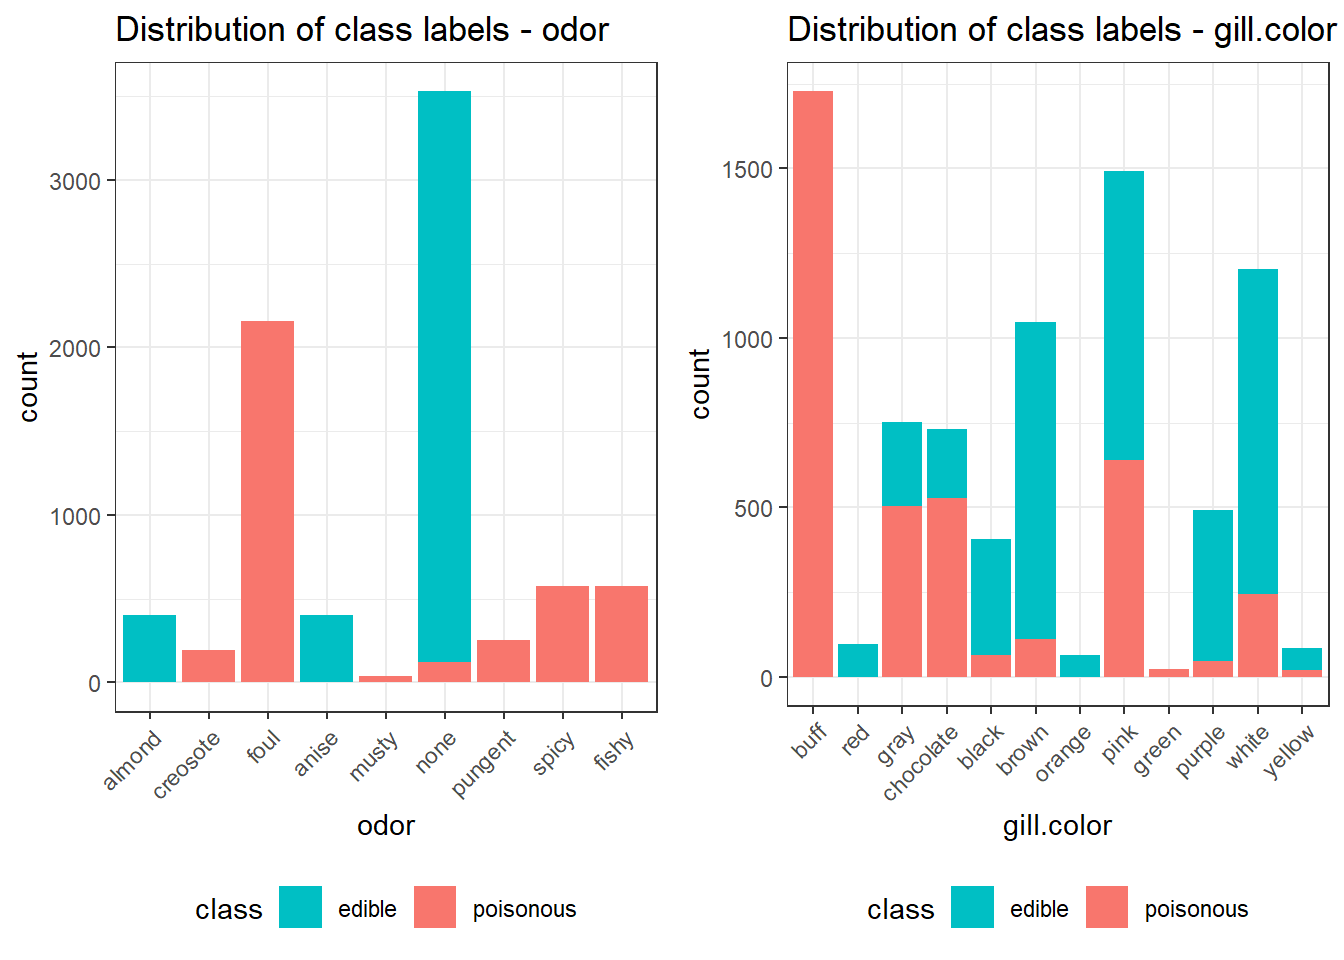
\includegraphics{präsi_files/figure-latex/unnamed-chunk-5-1.pdf}

\hypertarget{mushroom-learning}{%
\subsubsection{Mushroom Learning}\label{mushroom-learning}}

\hypertarget{evaluation-framework}{%
\paragraph{Evaluation Framework}\label{evaluation-framework}}

mlr3 is a machine learning (our in our case mushroom learning) framework
offering a common ground for all necessary steps as defining a task,
training a learner, predicting new data and resampling.\\
A task in mlr3 contains the data as well as meta information such as the
name of the target variable or if its a ``classification''
``regression'' task.

\begin{Shaded}
\begin{Highlighting}[]
\CommentTok{# Construct Classification Task }
\NormalTok{task_mushrooms =}\StringTok{ }\NormalTok{TaskClassif}\OperatorTok{$}\KeywordTok{new}\NormalTok{(}\DataTypeTok{id =} \StringTok{"mushrooms_data"}\NormalTok{,}
                               \DataTypeTok{backend =}\NormalTok{ mushrooms_data,}
                               \DataTypeTok{target =} \StringTok{"class"}\NormalTok{,}
                               \DataTypeTok{positive =} \StringTok{"e"}\NormalTok{) }\CommentTok{# "e" = edible}
\end{Highlighting}
\end{Shaded}

Additionally to building a machine learning model for predicting the
classes it is crucial to obtain an unbiased generalization error for our
estimates. Therefore we decided for a nested resampling strategy with a
5-fold CV in inner loop and a 10-fold CV in the outer loop. The number
of folds was chosen in a way to balance the bias and variance of our
estimate while still considering run time.

\begin{Shaded}
\begin{Highlighting}[]
\CommentTok{# Resampling Strategies }
\CommentTok{# 5 fold cross validation for inner loop}
\NormalTok{resampling_inner_5CV =}\StringTok{ }\KeywordTok{rsmp}\NormalTok{(}\StringTok{"cv"}\NormalTok{, }\DataTypeTok{folds =}\NormalTok{ 5L)}
\CommentTok{# 10 fold cross validation for outer loop}
\NormalTok{resampling_outer_10CV =}\StringTok{ }\KeywordTok{rsmp}\NormalTok{(}\StringTok{"cv"}\NormalTok{, }\DataTypeTok{folds =}\NormalTok{ 10L)}
\end{Highlighting}
\end{Shaded}

While model tuning will be solely based on the AUC, printing other
measures is useful for assessing the performances for the more relevant
error of falsely predicting a poisonous mushroom as edible.\\
Since the range of values of the hyperparameters is quite limited we
chose grid search for optimizing.

\begin{Shaded}
\begin{Highlighting}[]
\CommentTok{# Performance Measures }
\NormalTok{measures =}\StringTok{ }\KeywordTok{list}\NormalTok{(}
  \KeywordTok{msr}\NormalTok{(}\StringTok{"classif.auc"}\NormalTok{,}
      \DataTypeTok{id =} \StringTok{"AUC"}\NormalTok{),}
  \KeywordTok{msr}\NormalTok{(}\StringTok{"classif.fpr"}\NormalTok{,}
      \DataTypeTok{id =} \StringTok{"False Positive Rate"}\NormalTok{), }\CommentTok{# false positive rate especially interesting}
  \CommentTok{# for our falsely edible (although actually poisonous) classification}
  \KeywordTok{msr}\NormalTok{(}\StringTok{"classif.sensitivity"}\NormalTok{,}
      \DataTypeTok{id =} \StringTok{"Sensitivity"}\NormalTok{),}
  \KeywordTok{msr}\NormalTok{(}\StringTok{"classif.specificity"}\NormalTok{,}
      \DataTypeTok{id =} \StringTok{"Specificity"}\NormalTok{),}
  \KeywordTok{msr}\NormalTok{(}\StringTok{"classif.ce"}\NormalTok{, }
      \DataTypeTok{id =} \StringTok{"MMCE"}\NormalTok{)}
\NormalTok{)}

\CommentTok{# Choose optimization algorithm:}
\NormalTok{tuner_grid_search_knn =}\StringTok{ }\KeywordTok{tnr}\NormalTok{(}\StringTok{"grid_search"}\NormalTok{, }\DataTypeTok{resolution =} \DecValTok{50}\NormalTok{)}
\NormalTok{tuner_grid_search_mtry =}\StringTok{ }\KeywordTok{tnr}\NormalTok{(}\StringTok{"grid_search"}\NormalTok{, }\DataTypeTok{resolution =} \DecValTok{21}\NormalTok{)}

\CommentTok{# evaluate performance on AUC:}
\NormalTok{measures_tuning =}\StringTok{ }\KeywordTok{msr}\NormalTok{(}\StringTok{"classif.auc"}\NormalTok{, }\DataTypeTok{id =} \StringTok{"AUC"}\NormalTok{)}
\CommentTok{# Set when to terminate:}
\NormalTok{terminator_knn =}\StringTok{ }\KeywordTok{term}\NormalTok{(}\StringTok{"evals"}\NormalTok{, }\DataTypeTok{n_evals =} \DecValTok{50}\NormalTok{)}
\CommentTok{# since almost all mtry values lead to very good results we evaluate 1 to 21 features as opposed to a termination criterion like stagnation}
\NormalTok{terminator_mtry =}\StringTok{ }\KeywordTok{term}\NormalTok{(}\StringTok{"evals"}\NormalTok{, }\DataTypeTok{n_evals =} \DecValTok{21}\NormalTok{)  }
\end{Highlighting}
\end{Shaded}

\hypertarget{choosing-algorithms}{%
\paragraph{Choosing algorithms}\label{choosing-algorithms}}

A relevant property of our dataset is that all features are nominal and
thus multinomial distributed. Therefore linear and quadratic
discriminant analyses (LDA and QDA) are due to the violated assumption
of normally distributed features not possible.\\
Following the performance of featureless, naive bayes, KNN, logistic
regression, decision tree and random forest models will be compared.

In the following part we define our inner loop of nested resampling.
Only random forest (mtry) and KNN (k) have hyperparameters which will be
tuned in a 5-fold-cv.

\begin{Shaded}
\begin{Highlighting}[]
\CommentTok{# Autotune knn -----------------------------------------------------------------}
\CommentTok{# Define learner:}
\NormalTok{learner_knn =}\StringTok{ }\KeywordTok{lrn}\NormalTok{(}\StringTok{"classif.kknn"}\NormalTok{, }\DataTypeTok{predict_type =} \StringTok{"prob"}\NormalTok{)}

\CommentTok{# tune the chosen hyperparameter k with these boundaries:}
\NormalTok{param_k =}\StringTok{ }\NormalTok{ParamSet}\OperatorTok{$}\KeywordTok{new}\NormalTok{(}
  \KeywordTok{list}\NormalTok{(}
\NormalTok{    ParamInt}\OperatorTok{$}\KeywordTok{new}\NormalTok{(}\StringTok{"k"}\NormalTok{, }\DataTypeTok{lower =}\NormalTok{ 1L, }\DataTypeTok{upper =} \DecValTok{50}\NormalTok{)}
\NormalTok{  )}
\NormalTok{)}

\CommentTok{# Set up autotuner instance with the predefined setups}
\NormalTok{tuner_knn =}\StringTok{ }\NormalTok{AutoTuner}\OperatorTok{$}\KeywordTok{new}\NormalTok{(}
  \DataTypeTok{learner =}\NormalTok{ learner_knn,}
  \DataTypeTok{resampling =}\NormalTok{ resampling_inner_5CV,}
  \DataTypeTok{measures =}\NormalTok{ measures_tuning, }
  \DataTypeTok{tune_ps =}\NormalTok{ param_k, }
  \DataTypeTok{terminator =}\NormalTok{ terminator_knn,}
  \DataTypeTok{tuner =}\NormalTok{ tuner_grid_search_knn}
\NormalTok{)}



\CommentTok{# Autotune Random Forest ---------------------------------------------------------------------------}
\CommentTok{# Define learner:}
\NormalTok{learner_ranger =}\StringTok{ }\KeywordTok{lrn}\NormalTok{(}\StringTok{"classif.ranger"}\NormalTok{, }\DataTypeTok{predict_type =} \StringTok{"prob"}\NormalTok{, }\DataTypeTok{importance =} \StringTok{"impurity"}\NormalTok{)}


\CommentTok{# we will try all configurations: 1 to 21 features.}
\NormalTok{param_mtry =}\StringTok{ }\NormalTok{ParamSet}\OperatorTok{$}\KeywordTok{new}\NormalTok{(}
  \KeywordTok{list}\NormalTok{(}
\NormalTok{    ParamInt}\OperatorTok{$}\KeywordTok{new}\NormalTok{(}\StringTok{"mtry"}\NormalTok{, }\DataTypeTok{lower =}\NormalTok{ 1L, }\DataTypeTok{upper =}\NormalTok{ 21L)}
\NormalTok{  ) }
\NormalTok{)}

\CommentTok{# Set up autotuner instance with the predefined setups}
\NormalTok{tuner_ranger =}\StringTok{ }\NormalTok{AutoTuner}\OperatorTok{$}\KeywordTok{new}\NormalTok{(}
  \DataTypeTok{learner =}\NormalTok{ learner_ranger,}
  \DataTypeTok{resampling =}\NormalTok{ resampling_inner_5CV,}
  \DataTypeTok{measures =}\NormalTok{ measures_tuning,}
  \DataTypeTok{tune_ps =}\NormalTok{ param_mtry, }
  \DataTypeTok{terminator =}\NormalTok{ terminator_mtry,}
  \DataTypeTok{tuner =}\NormalTok{ tuner_grid_search_mtry}
\NormalTok{)}


\NormalTok{(}\DataTypeTok{learners =} \KeywordTok{list}\NormalTok{(}\KeywordTok{lrn}\NormalTok{(}\StringTok{"classif.featureless"}\NormalTok{, }\DataTypeTok{predict_type =} \StringTok{"prob"}\NormalTok{),}
                \KeywordTok{lrn}\NormalTok{(}\StringTok{"classif.naive_bayes"}\NormalTok{, }\DataTypeTok{predict_type =} \StringTok{"prob"}\NormalTok{),}
                \KeywordTok{lrn}\NormalTok{(}\StringTok{"classif.rpart"}\NormalTok{, }\DataTypeTok{predict_type =} \StringTok{"prob"}\NormalTok{),}
                \KeywordTok{lrn}\NormalTok{(}\StringTok{"classif.log_reg"}\NormalTok{, }\DataTypeTok{predict_type =} \StringTok{"prob"}\NormalTok{),}
\NormalTok{                tuner_ranger,}
\NormalTok{                tuner_knn))}
\end{Highlighting}
\end{Shaded}

\begin{verbatim}
## [[1]]
## <LearnerClassifFeatureless:classif.featureless>
## * Model: -
## * Parameters: method=mode
## * Packages: -
## * Predict Type: prob
## * Feature types: logical, integer, numeric, character, factor, ordered
## * Properties: importance, missings, multiclass, selected_features,
##   twoclass
## 
## [[2]]
## <LearnerClassifNaiveBayes:classif.naive_bayes>
## * Model: -
## * Parameters: list()
## * Packages: e1071
## * Predict Type: prob
## * Feature types: logical, integer, numeric, factor
## * Properties: multiclass, twoclass
## 
## [[3]]
## <LearnerClassifRpart:classif.rpart>
## * Model: -
## * Parameters: xval=0
## * Packages: rpart
## * Predict Type: prob
## * Feature types: logical, integer, numeric, factor, ordered
## * Properties: importance, missings, multiclass, selected_features,
##   twoclass, weights
## 
## [[4]]
## <LearnerClassifLogReg:classif.log_reg>
## * Model: -
## * Parameters: list()
## * Packages: stats
## * Predict Type: prob
## * Feature types: logical, integer, numeric, character, factor, ordered
## * Properties: twoclass, weights
## 
## [[5]]
## <AutoTuner:classif.ranger.tuned>
## * Model: -
## * Parameters: importance=impurity
## * Packages: ranger
## * Predict Type: prob
## * Feature types: logical, integer, numeric, character, factor, ordered
## * Properties: importance, multiclass, oob_error, twoclass, weights
## 
## [[6]]
## <AutoTuner:classif.kknn.tuned>
## * Model: -
## * Parameters: list()
## * Packages: kknn
## * Predict Type: prob
## * Feature types: logical, integer, numeric, factor, ordered
## * Properties: multiclass, twoclass
\end{verbatim}

\hypertarget{results}{%
\paragraph{Results}\label{results}}

Here the outer loop of nested resampling is done with a 10-fold-cv.

\begin{Shaded}
\begin{Highlighting}[]
\NormalTok{design =}\StringTok{ }\KeywordTok{benchmark_grid}\NormalTok{(}
  \DataTypeTok{tasks =}\NormalTok{ task_mushrooms,}
  \DataTypeTok{learners =}\NormalTok{ learners,}
  \DataTypeTok{resamplings =}\NormalTok{ resampling_outer_10CV}
\NormalTok{)}



\CommentTok{#lower the threshold to only print warnings:}
\NormalTok{lgr}\OperatorTok{::}\KeywordTok{get_logger}\NormalTok{(}\StringTok{"mlr3"}\NormalTok{)}\OperatorTok{$}\KeywordTok{set_threshold}\NormalTok{(}\StringTok{"warn"}\NormalTok{)}

\NormalTok{bmr =}\StringTok{ }\KeywordTok{benchmark}\NormalTok{(design, }\DataTypeTok{store_models =} \OtherTok{TRUE}\NormalTok{)}
\end{Highlighting}
\end{Shaded}

\begin{verbatim}
## Warning: glm.fit: algorithm did not converge
\end{verbatim}

\begin{verbatim}
## Warning in predict.lm(object, newdata, se.fit, scale = 1, type = if (type == :
## prediction from a rank-deficient fit may be misleading
\end{verbatim}

\begin{verbatim}
## Warning: glm.fit: algorithm did not converge
\end{verbatim}

\begin{verbatim}
## Warning in predict.lm(object, newdata, se.fit, scale = 1, type = if (type == :
## prediction from a rank-deficient fit may be misleading
\end{verbatim}

\begin{verbatim}
## Warning: glm.fit: algorithm did not converge
\end{verbatim}

\begin{verbatim}
## Warning in predict.lm(object, newdata, se.fit, scale = 1, type = if (type == :
## prediction from a rank-deficient fit may be misleading
\end{verbatim}

\begin{verbatim}
## Warning: glm.fit: algorithm did not converge
\end{verbatim}

\begin{verbatim}
## Warning in predict.lm(object, newdata, se.fit, scale = 1, type = if (type == :
## prediction from a rank-deficient fit may be misleading
\end{verbatim}

\begin{verbatim}
## Warning: glm.fit: algorithm did not converge
\end{verbatim}

\begin{verbatim}
## Warning in predict.lm(object, newdata, se.fit, scale = 1, type = if (type == :
## prediction from a rank-deficient fit may be misleading
\end{verbatim}

\begin{verbatim}
## Warning: glm.fit: algorithm did not converge
\end{verbatim}

\begin{verbatim}
## Warning in predict.lm(object, newdata, se.fit, scale = 1, type = if (type == :
## prediction from a rank-deficient fit may be misleading
\end{verbatim}

\begin{verbatim}
## Warning: glm.fit: algorithm did not converge
\end{verbatim}

\begin{verbatim}
## Warning in predict.lm(object, newdata, se.fit, scale = 1, type = if (type == :
## prediction from a rank-deficient fit may be misleading
\end{verbatim}

\begin{verbatim}
## Warning: glm.fit: algorithm did not converge
\end{verbatim}

\begin{verbatim}
## Warning in predict.lm(object, newdata, se.fit, scale = 1, type = if (type == :
## prediction from a rank-deficient fit may be misleading
\end{verbatim}

\begin{verbatim}
## Warning: glm.fit: algorithm did not converge
\end{verbatim}

\begin{verbatim}
## Warning in predict.lm(object, newdata, se.fit, scale = 1, type = if (type == :
## prediction from a rank-deficient fit may be misleading
\end{verbatim}

\begin{verbatim}
## Warning: glm.fit: algorithm did not converge
\end{verbatim}

\begin{verbatim}
## Warning in predict.lm(object, newdata, se.fit, scale = 1, type = if (type == :
## prediction from a rank-deficient fit may be misleading
\end{verbatim}

\begin{Shaded}
\begin{Highlighting}[]
\CommentTok{# reset to default:}
\NormalTok{lgr}\OperatorTok{::}\KeywordTok{get_logger}\NormalTok{(}\StringTok{"mlr3"}\NormalTok{)}\OperatorTok{$}\KeywordTok{set_threshold}\NormalTok{(}\StringTok{"info"}\NormalTok{)}
\end{Highlighting}
\end{Shaded}

First of all we see that no errors or warnings occurred during
resampling when printing the benchmark result print(bmr).

\begin{Shaded}
\begin{Highlighting}[]
\KeywordTok{print}\NormalTok{(bmr)}
\end{Highlighting}
\end{Shaded}

\begin{verbatim}
## <BenchmarkResult> of 60 rows with 6 resampling runs
##  nr        task_id           learner_id resampling_id iters warnings errors
##   1 mushrooms_data  classif.featureless            cv    10        0      0
##   2 mushrooms_data  classif.naive_bayes            cv    10        0      0
##   3 mushrooms_data        classif.rpart            cv    10        0      0
##   4 mushrooms_data      classif.log_reg            cv    10        0      0
##   5 mushrooms_data classif.ranger.tuned            cv    10        0      0
##   6 mushrooms_data   classif.kknn.tuned            cv    10        0      0
\end{verbatim}

As expected a featureless model stays at a classification error of close
to 0.5.

\begin{Shaded}
\begin{Highlighting}[]
\KeywordTok{autoplot}\NormalTok{(bmr)}
\end{Highlighting}
\end{Shaded}

\includegraphics{präsi_files/figure-latex/unnamed-chunk-12-1.pdf}

\begin{Shaded}
\begin{Highlighting}[]
\KeywordTok{autoplot}\NormalTok{(bmr, }\DataTypeTok{type =} \StringTok{"roc"}\NormalTok{)}
\end{Highlighting}
\end{Shaded}

\includegraphics{präsi_files/figure-latex/unnamed-chunk-12-2.pdf}

\begin{Shaded}
\begin{Highlighting}[]
\NormalTok{(}\DataTypeTok{tab_learner_performance =}\NormalTok{ bmr}\OperatorTok{$}\KeywordTok{aggregate}\NormalTok{(measures))}
\end{Highlighting}
\end{Shaded}

\begin{verbatim}
##    nr  resample_result        task_id           learner_id resampling_id iters
## 1:  1 <ResampleResult> mushrooms_data  classif.featureless            cv    10
## 2:  2 <ResampleResult> mushrooms_data  classif.naive_bayes            cv    10
## 3:  3 <ResampleResult> mushrooms_data        classif.rpart            cv    10
## 4:  4 <ResampleResult> mushrooms_data      classif.log_reg            cv    10
## 5:  5 <ResampleResult> mushrooms_data classif.ranger.tuned            cv    10
## 6:  6 <ResampleResult> mushrooms_data   classif.kknn.tuned            cv    10
##          AUC False Positive Rate Sensitivity Specificity         MMCE
## 1: 0.5000000        1.0000000000    1.000000   0.0000000 0.4820289447
## 2: 0.9960508        0.1156206472    0.993594   0.8843794 0.0589604578
## 3: 0.9938725        0.0122550286    1.000000   0.9877450 0.0059081490
## 4: 1.0000000        0.0000000000    1.000000   1.0000000 0.0000000000
## 5: 1.0000000        0.0000000000    1.000000   1.0000000 0.0000000000
## 6: 1.0000000        0.0002564103    1.000000   0.9997436 0.0001231527
\end{verbatim}

Logistic regression and random forest clearly lead to the best results
when ranking the different models by their AUC.

\begin{Shaded}
\begin{Highlighting}[]
\NormalTok{learner_performance_ranked <-}\StringTok{ }\NormalTok{tab_learner_performance[,}
\NormalTok{                                                      .(learner_id,}
                                                        \DataTypeTok{rank_train =} \KeywordTok{rank}\NormalTok{(}\OperatorTok{-}\NormalTok{AUC),}
                                                        \DataTypeTok{rank_test =} \KeywordTok{rank}\NormalTok{(MMCE))}
\NormalTok{                                                      ] }\OperatorTok\StringTok{ }
\StringTok{  }\KeywordTok{arrange}\NormalTok{(rank_train) }\CommentTok{# sort in ascending order}
\NormalTok{learner_performance_ranked}
\end{Highlighting}
\end{Shaded}

\begin{verbatim}
##             learner_id rank_train rank_test
## 1      classif.log_reg          2       1.5
## 2 classif.ranger.tuned          2       1.5
## 3   classif.kknn.tuned          2       3.0
## 4  classif.naive_bayes          4       5.0
## 5        classif.rpart          5       4.0
## 6  classif.featureless          6       6.0
\end{verbatim}

\hypertarget{final-model}{%
\subsubsection{Final model}\label{final-model}}

All steps so far answered the question which model with which
hyperparameters yields good results with a now known generalization
error. However to obtain the best possible model, training with all
available data points is needed. We chose the random forest as final
model for its interpretability and stability.

\begin{Shaded}
\begin{Highlighting}[]
\CommentTok{# Train tuner_ranger once again using the same specs as before}
\NormalTok{tuner_ranger}\OperatorTok{$}\NormalTok{tuning_instance}

\CommentTok{# show only warnings:}
\NormalTok{lgr}\OperatorTok{::}\KeywordTok{get_logger}\NormalTok{(}\StringTok{"mlr3"}\NormalTok{)}\OperatorTok{$}\KeywordTok{set_threshold}\NormalTok{(}\StringTok{"warn"}\NormalTok{)}
\NormalTok{tuner_ranger}\OperatorTok{$}\KeywordTok{train}\NormalTok{(task_mushrooms)}
\CommentTok{# reset console outputs to default:}
\NormalTok{lgr}\OperatorTok{::}\KeywordTok{get_logger}\NormalTok{(}\StringTok{"mlr3"}\NormalTok{)}\OperatorTok{$}\KeywordTok{set_threshold}\NormalTok{(}\StringTok{"info"}\NormalTok{)}

\CommentTok{# AUC performance for parameter combinations:}
\NormalTok{tuner_ranger}\OperatorTok{$}\NormalTok{tuning_instance}\OperatorTok{$}\KeywordTok{archive}\NormalTok{(}\DataTypeTok{unnest =} \StringTok{"params"}\NormalTok{)[,}
                                                        \KeywordTok{c}\NormalTok{(}\StringTok{"mtry"}\NormalTok{,}\StringTok{"AUC"}\NormalTok{)] }\OperatorTok\StringTok{ }
\StringTok{  }\KeywordTok{arrange}\NormalTok{(mtry)}
\CommentTok{# Pretty much every combination works perfectly}

\NormalTok{tuner_ranger}\OperatorTok{$}\NormalTok{tuning_result }\CommentTok{# winning mtry is 3 although we could use}
\CommentTok{# 2-21 and achieve the same perfect performance}

\CommentTok{# use these parameters for our final winner model with winner specs:}
\NormalTok{learner_final =}\StringTok{ }\KeywordTok{lrn}\NormalTok{(}\StringTok{"classif.ranger"}\NormalTok{,}\DataTypeTok{predict_type =} \StringTok{"prob"}\NormalTok{)}
\NormalTok{learner_final}\OperatorTok{$}\NormalTok{param_set}\OperatorTok{$}\NormalTok{values =}\StringTok{ }\NormalTok{tuner_ranger}\OperatorTok{$}\NormalTok{tuning_result}\OperatorTok{$}\NormalTok{params}

\CommentTok{# Fit winner model to entire data set}
\NormalTok{learner_final}\OperatorTok{$}\KeywordTok{train}\NormalTok{(task_mushrooms)}
\end{Highlighting}
\end{Shaded}

With random forests we can asses the importance of each variable in the
data. As suspected in the description part odor is clearly a good
indicator for edibility of a mushroom.

\begin{Shaded}
\begin{Highlighting}[]
\CommentTok{# construct filter to extract variable importance in previously set up winning learner}
\NormalTok{filter_ranger =}\StringTok{ }\KeywordTok{flt}\NormalTok{(}\StringTok{"importance"}\NormalTok{, }\DataTypeTok{learner =}\NormalTok{ learner_final)}
\CommentTok{# rerun learner on entire data set and store variable importance results}
\NormalTok{filter_ranger}\OperatorTok{$}\KeywordTok{calculate}\NormalTok{(task_mushrooms)}

\NormalTok{feature_scores <-}\StringTok{ }\KeywordTok{as.data.table}\NormalTok{(filter_ranger)}

\KeywordTok{ggplot}\NormalTok{(}\DataTypeTok{data =}\NormalTok{ feature_scores, }
       \KeywordTok{aes}\NormalTok{(}\DataTypeTok{x =} \KeywordTok{reorder}\NormalTok{(feature, }\OperatorTok{-}\NormalTok{score),}
           \DataTypeTok{y =}\NormalTok{ score)) }\OperatorTok{+}
\StringTok{  }\KeywordTok{geom_bar}\NormalTok{(}\DataTypeTok{stat =} \StringTok{"identity"}\NormalTok{) }\OperatorTok{+}
\StringTok{  }\KeywordTok{ggtitle}\NormalTok{(}\DataTypeTok{label =} \StringTok{"Mushroom Features - Variable Importance in Random Forest"}\NormalTok{) }\OperatorTok{+}
\StringTok{  }\KeywordTok{labs}\NormalTok{(}\DataTypeTok{x =} \StringTok{"Features"}\NormalTok{, }\DataTypeTok{y =} \StringTok{"Variable Importance Score"}\NormalTok{) }\OperatorTok{+}
\StringTok{  }\KeywordTok{theme}\NormalTok{(}\DataTypeTok{axis.text.x =} \KeywordTok{element_text}\NormalTok{(}\DataTypeTok{angle =} \DecValTok{45}\NormalTok{, }\DataTypeTok{hjust =} \DecValTok{1}\NormalTok{))}\OperatorTok{+}
\StringTok{  }\KeywordTok{scale_y_continuous}\NormalTok{(}\DataTypeTok{breaks =} \KeywordTok{pretty}\NormalTok{(}\DecValTok{1}\OperatorTok{:}\NormalTok{feature_scores}\OperatorTok{$}\NormalTok{score[}\DecValTok{1}\NormalTok{],}\DecValTok{10}\NormalTok{))}
\end{Highlighting}
\end{Shaded}

\includegraphics{präsi_files/figure-latex/unnamed-chunk-15-1.pdf}

\end{document}
